\null\newpage
\clearpage

\section{Anexo}

\subsection{Diseno final - imágenes}
\begin{figure}[htb]
    \centering
    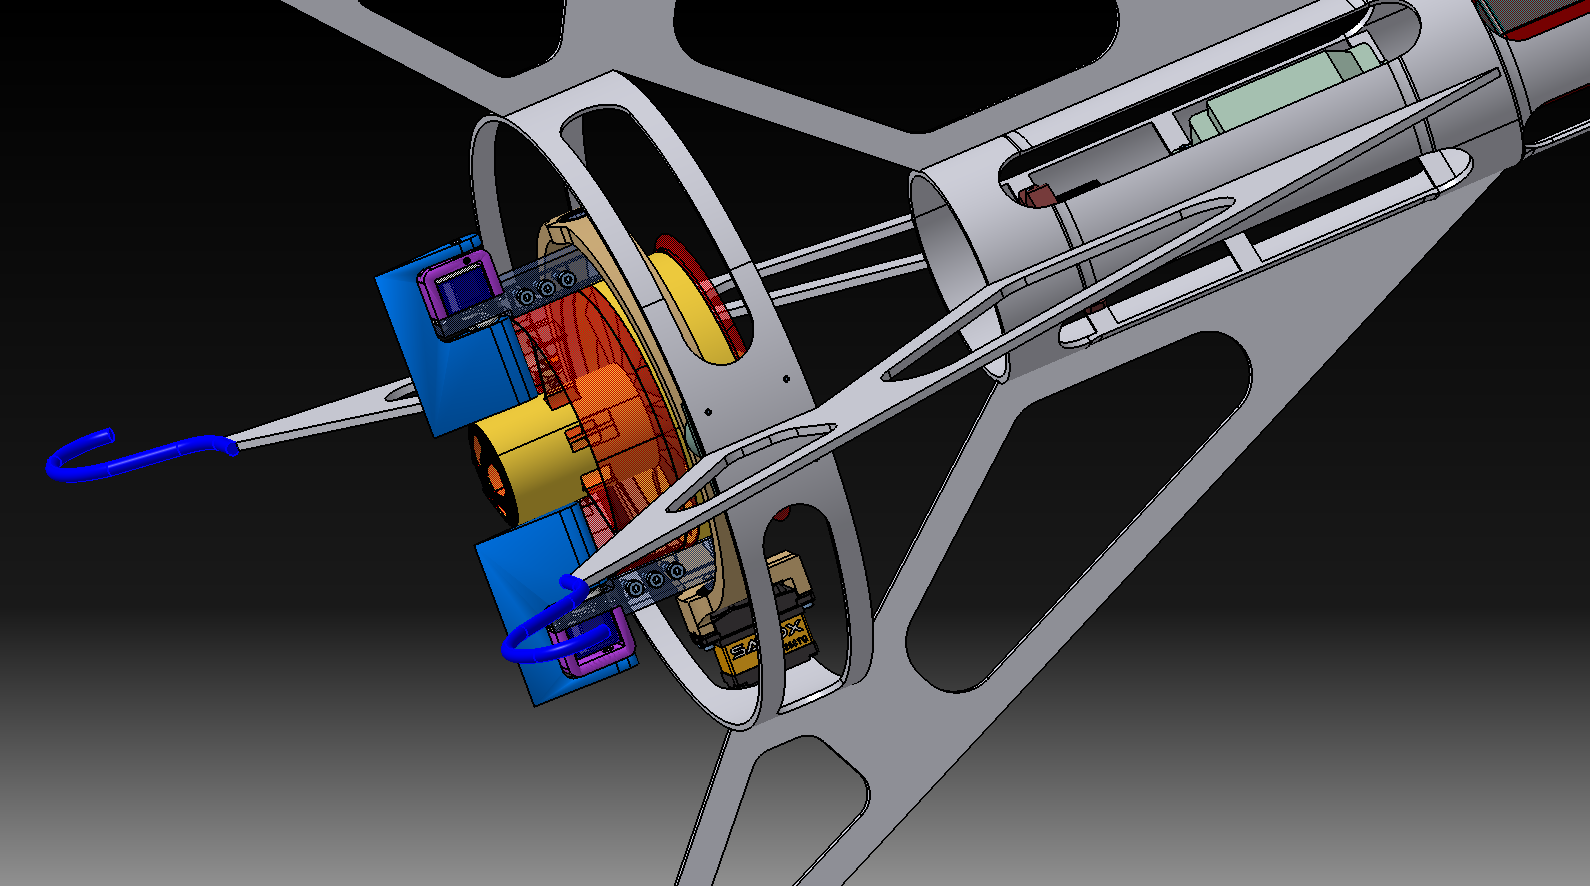
\includegraphics[width=\linewidth]{fig/design/v6_3}
    \caption{Prototipo final detalle EDF.}
    \label{fig:design/v6_3}
\end{figure}

\begin{figure}[htb]
    \centering
    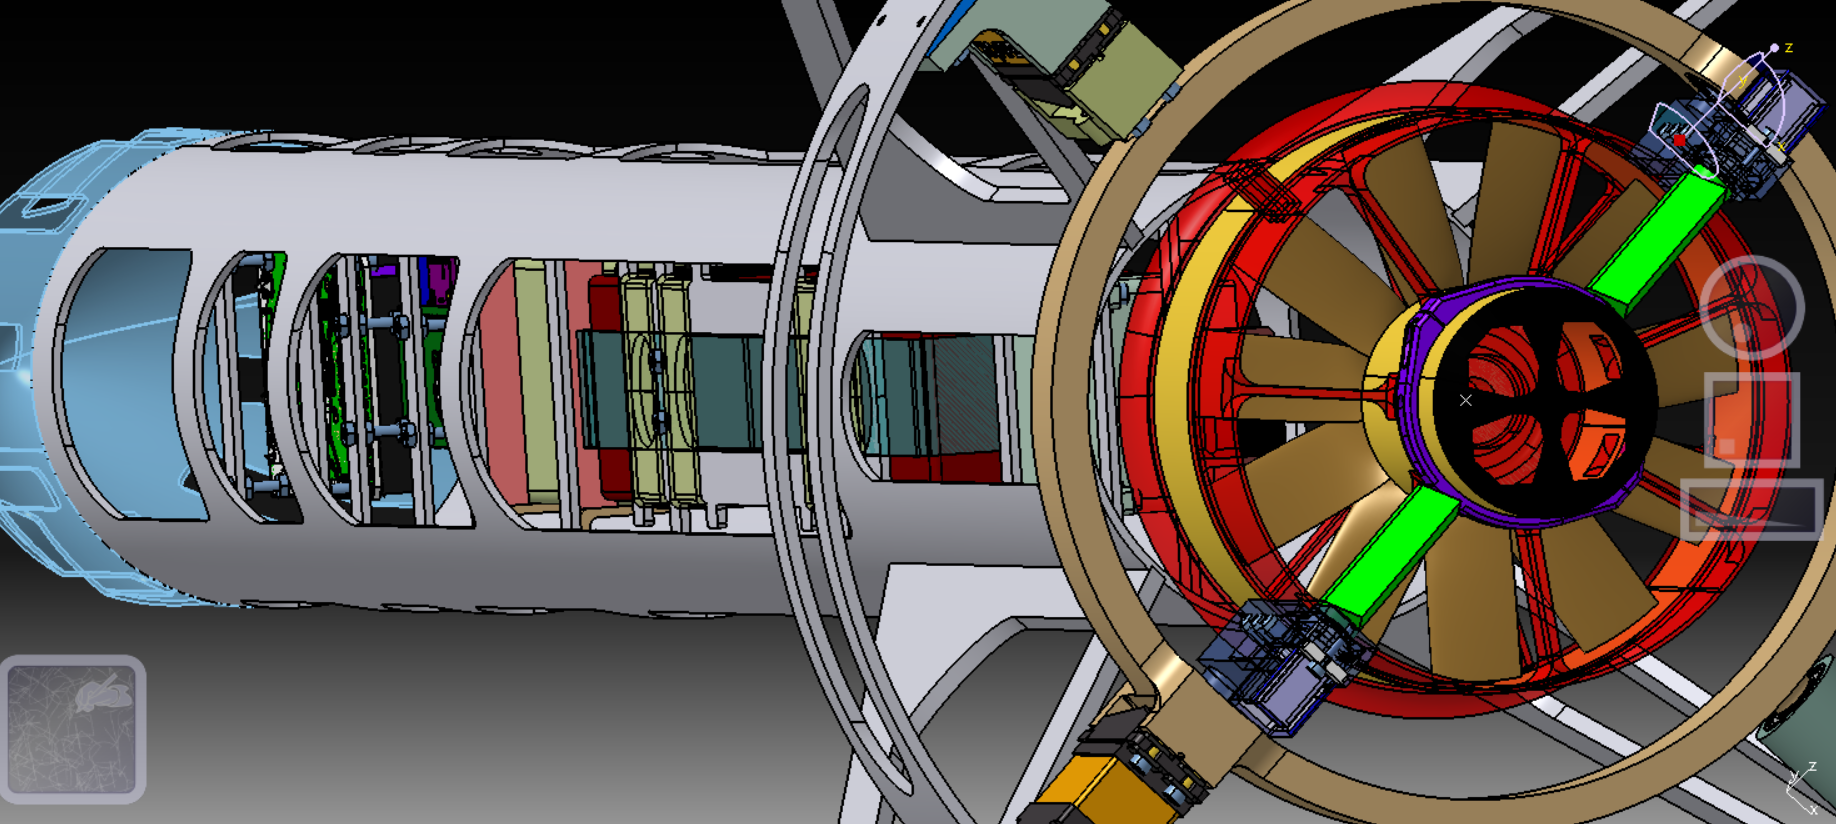
\includegraphics[width=\linewidth]{fig/design/v6_5}
    \caption{Prototipo final vista inferior detalle constructivo.}
    \label{fig:design/v6_5}
\end{figure}

\subsection{Diseños preliminares - imágenes}

\begin{figure}[htb]
    \centering
    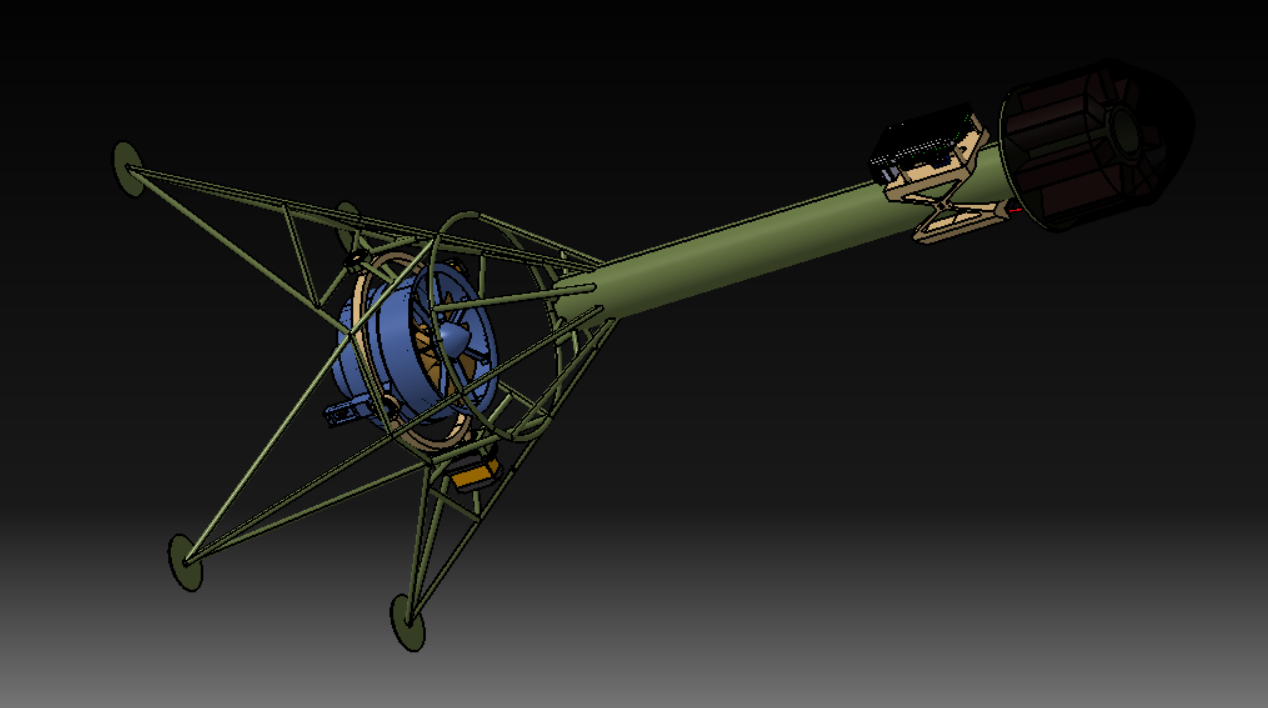
\includegraphics[width=\linewidth]{fig/design/0}
    \caption{Prototipo de fuselaje con patas reticuladas integro en aluminio, baterías en la nariz, aviónica debajo de la nariz, sin sistema anti rolido.}
    \label{fig:design/0}
\end{figure}


\begin{figure}[htb]
    \centering
    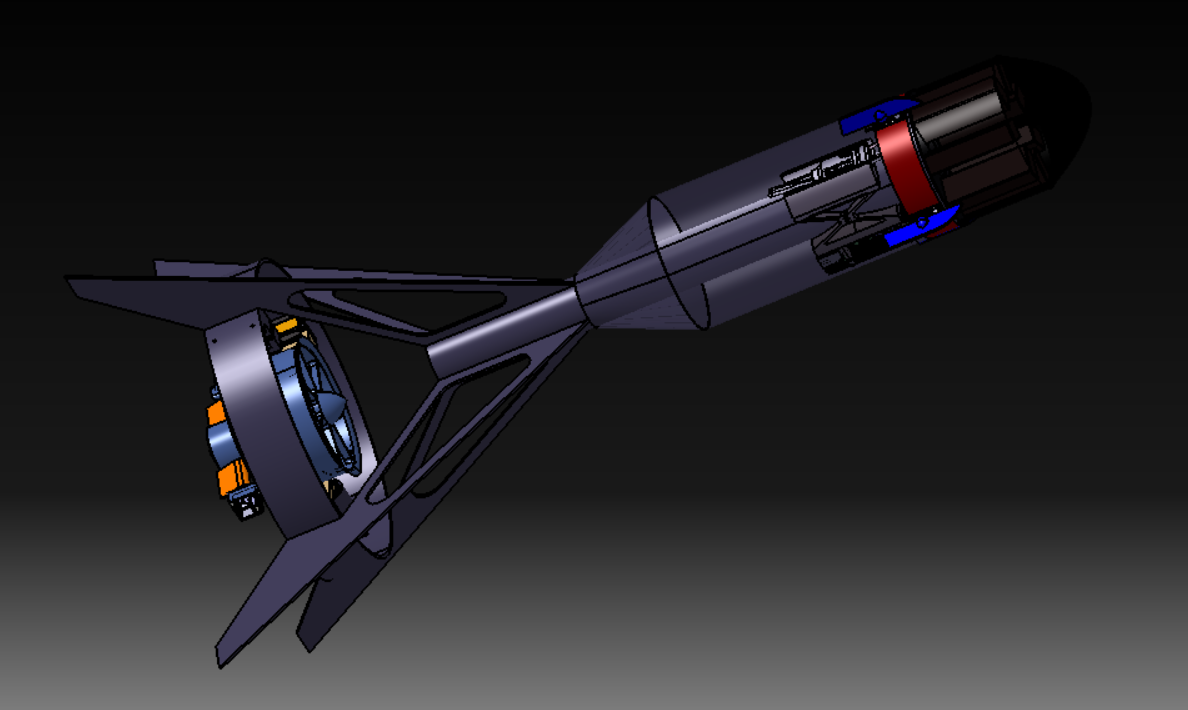
\includegraphics[width=\linewidth]{fig/design/1}
    \caption{Prototipo evolución al fuselaje de aluminio tubular, baterías en la nariz, sistema anti rolido en
    la parte superior, aviónica debajo de las baterías.}
    \label{fig:design/1}
\end{figure}

\begin{figure}[htb]
    \centering
    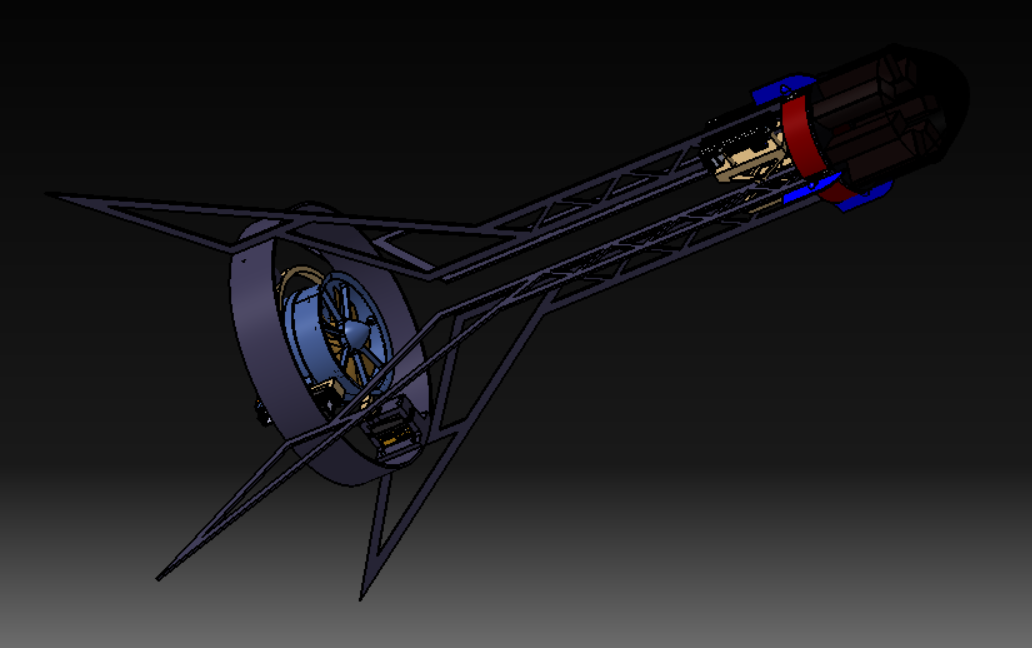
\includegraphics[width=\linewidth]{fig/design/2}
    \caption{Prototipo fuselaje reticulado de aluminio en forma de placas, baterías en la nariz, sistema anti
    rolido en la parte superior, aviónica debajo de las baterías.}
    \label{fig:design/2}
\end{figure}

\begin{figure}[htb]
    \centering
    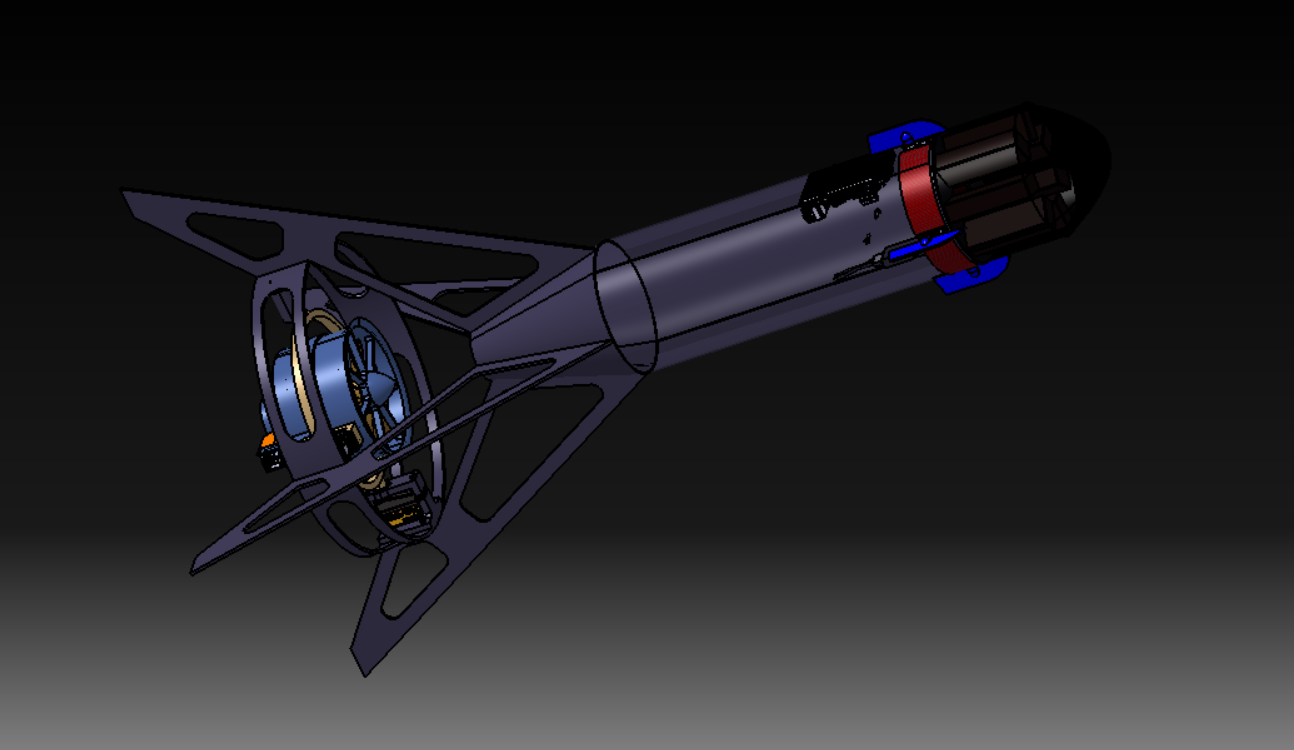
\includegraphics[width=\linewidth]{fig/design/3}
    \caption{Prototipo fuselaje reticulado de aluminio en forma de placas, baterías en la nariz, sistema anti
    rolido en la parte superior, aviónica debajo de las baterías.}
    \label{fig:design/3}
\end{figure}

\begin{figure}[htb]
    \centering
    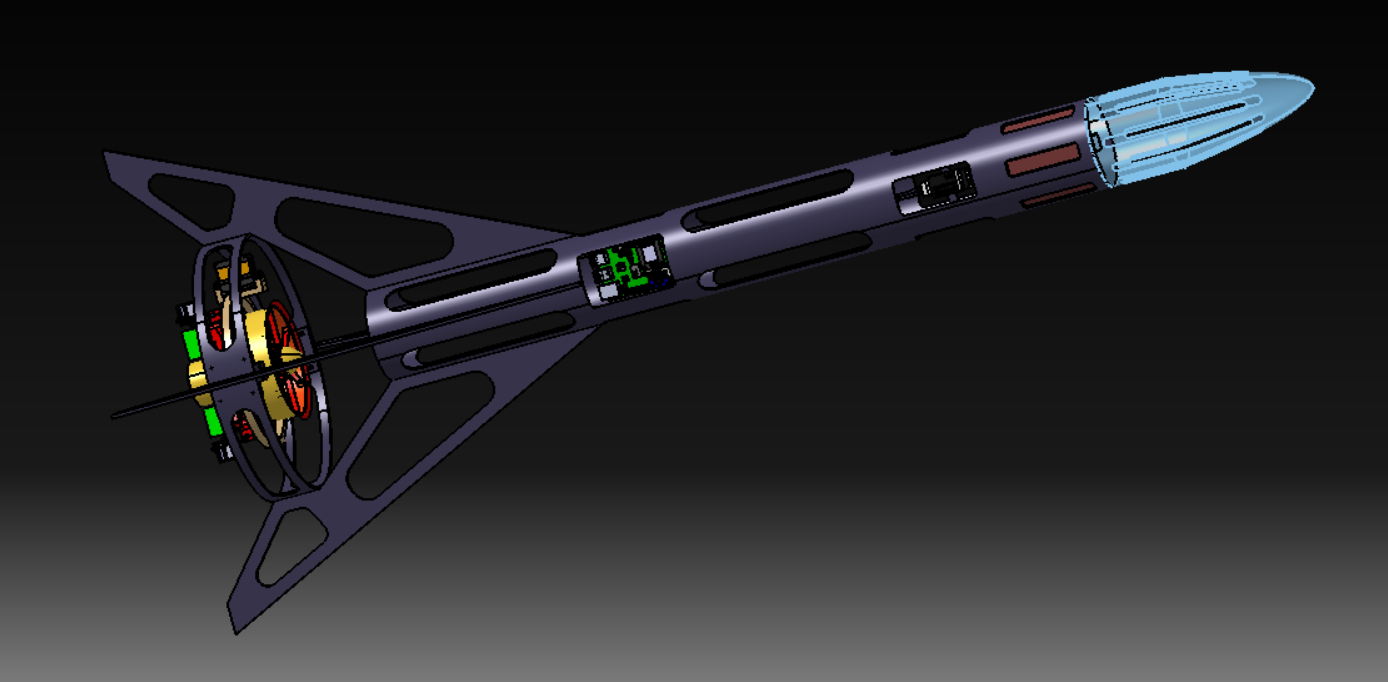
\includegraphics[width=\linewidth]{fig/design/4}
    \caption{Prototipo fuselaje de aluminio tubular vaciado, baterías en el cuerpo, en la parte superior, nariz
    aerodinámica, patas optimizadas, aviónica en la parte inferior, sistema anti-rolido en la parte
    inferior del EDF por derivación del flujo.}
    \label{fig:design/4}
\end{figure}


\begin{figure}[htb]
    \centering
    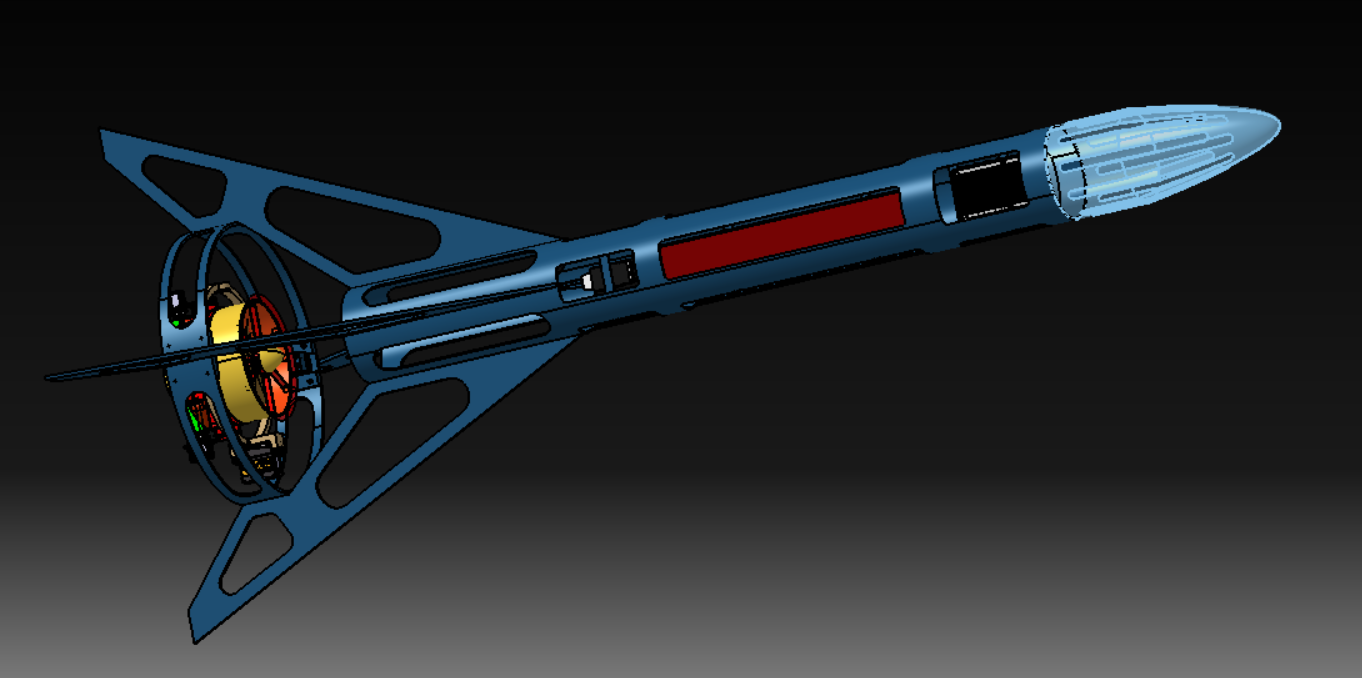
\includegraphics[width=\linewidth]{fig/design/5}
    \caption{Prototipo fuselaje de aluminio tubular vaciado, baterías en el cuerpo, en el núcleo, nariz aerodinámica, patas optimizadas, aviónica en la parte superior, sistema anti-rolido en la parte
    inferior del EDF por derivación del flujo.}
    \label{fig:design/5}
\end{figure}

\null\newpage
\clearpage

\subsection{Dinámica angular del vehículo} \label{ssec:ecuacionangular}


El momento angular del vehículo respecto de su centro de masa ($\ogn{C}$) y representado en el marco fijo-tierra $\frm{N}$ debe tomar en cuenta el momento angular por tener un cuerpo con velocidad lineal y angular propia. 

\begin{equation}
		L_{\ogn{C}}^{\frm{N}} = \underbrace{\transform{{NB}} \cdot J_{\ogn{C}}^{\frm{B}} \cdot \omega_{\frm{BN}}^{\frm{B}}}_{\text{Vehículo}} + \underbrace{\transform{{NG}}J_{\!g\ogn{R}}^{\frm{G}} \cdot \omega_\frm{GN}^\frm{G} +
		 m_{g}\cdot \skw{\avec{r}}^\frm{N}_\ogn{RC} \cdot\dot{\avec{r}}^\frm{N}_\ogn{RC} }_\text{Cardán \& EDF} + \underbrace{ \transform{NG} \cdot J_{\!r\ogn{R}}^\frm{G} \cdot \omega_{\!r}^\frm{G} + m_{r}\cdot \skw{\avec{r}}^\frm{N}_\ogn{RC} \cdot\dot{\avec{r}}^\frm{N}_\ogn{RC}}_\text{Rotor}
\end{equation}

Esta ecuación describe los efectos de tener un cardán con un rotor integrado acoplado al vehículo sin embargo algunos términos se podrían considerar despreciables debido al diseño del cardán. 

Ambos gimbals del cardán tienen su eje de giro cercano a su centro de masa lo cual significa que la velocidad relativa entre los puntos $\ogn{R}$ y $\ogn{C}$ va tener poco impacto sobre los torques internos del vehículo. Se considera que
\begin{equation}
\dot{\avec{r}}_\ogn{RC}  = 0
\end{equation}

La velocidad angular de los gimbals es poca ya que su actuación ocurre en el orden de la décima de grado lo cual implica un bajo impacto del término del cardán cuando es integrado en el tiempo. El término  $\transform{{NG}}J_{\!g\ogn{R}}^{\frm{G}} \cdot \omega_\frm{GN}^\frm{G}$ entonces pasa a formar parte de la inercia del resto del vehículo $\inertia{C}{B}$, el cual ahora solo excluye al rotor.



El momento angular nos queda simplificado:


\begin{equation}
	L_{\ogn{C}}^{\frm{N}} = \transform{{NB}} \cdot \inertia{C}{B} \cdot \omega_{\frm{BN}}^{\frm{B}} +\transform{NG} \inertiarotor{R}{G} \cdot \omega_{\!r}^\frm{G}
\end{equation}
donde $\omega_{\!r}$ es la velocidad del rotor y $\inertiarotor{R}{G}$ es la matriz de inercia del rotor tomado alrededor de su centro de masa representado en coordenadas del marco cardán $\frm{G}$.


Derivamos el momento angular con respecto a $\frm{N}$ y junto con $\inertia{C}{B} \approx \text{constante}$ \footnote{La inercia del vehículo en su propio marco $\inertia{C}{B}$ es constante excepto por las variaciones introducidas al agruparlo con el término del cardán $J_{\!g\ogn{C}}^\frm{B}$, el cual varía en función a la actuación $\alpha,\beta$.}

\begin{IEEEeqnarray*}{rCl}
	\hspace{-1cm}
^{\frm{N}}\dot{L}_{\ogn{C}}^{\frm{N}}  & = & ^{\frm{N}} \frac{\di }{\di t}  \left(\transform{{NB}} \cdot \inertia{C}{B} \cdot \omega_{\frm{BN}}^{\frm{B}} + \transform{{NG}}\cdot \inertiarotor{R}{G} \cdot \omega_r^\frm{G} \right) \\
 & = & \dottransform{NB} \cdot\inertia{C}{B}\cdot \omega_{\frm{BN}}^{\frm{B}} + 
 \transform{{NB}} \cdot \underbrace{ {}^\frm{N}\dot{J}_{\ogn{C}}^\frm{B}}_{\approx 0}\cdot \omega_{\frm{BN}}^{\frm{B}} +
  \transform{{NB}} \cdot \inertia{C}{B}\cdot \dot{\omega}_{\frm{BN}}^{\frm{B}} + 
  \dottransform{NG}\cdot  \inertiarotor{R}{G} \cdot \omega_{\!r}^\frm{G} +
  \transform{{NG}}\cdot {}^\frm{N}\frac{\di}{\di t}\left( \inertiarotor{R}{G}  \cdot \omega_r^\frm{G} \right)
\end{IEEEeqnarray*}
la derivada de la inercia del cuerpo se anula y luego se aplica la regla de la cadena a la derivada
%\transform{{NG}}\cdot {}^\frm{N}\frac{\di}{\di t}\left( \inertiarotor{R}{G}  \cdot \omega_r^\frm{G} \right)
\begin{IEEEeqnarray*}{rCl}
	\hspace{-1cm}
^{\frm{N}}\dot{L}_{\ogn{C}}^{\frm{N}}  &=&\dottransform{NB} \cdot J_{\ogn{C}}^\frm{B}\cdot \omega_{\frm{BN}}^{\frm{B}} + 
\transform{{NB}} \cdot \inertia{C}{B}\cdot \dot{\omega}_{\frm{BN}}^{\frm{B}} + 
\dottransform{NG}\cdot \inertiarotor{R}{G}  \cdot \omega_r^\frm{G} +
\transform{{NG}}\cdot {}^\frm{N}\frac{\di}{\di t}\left( \inertiarotor{R}{G}  \cdot \omega_r^\frm{G} \right) \\
&=&\transform{{NB}} \cdot \skw{\omega}_\frm{BN}^\frm{B} \cdot \inertia{C}{B} \cdot \omega_{\frm{BN}}^{\frm{B}} + 
\transform{{NB}} \cdot \inertia{C}{B}\cdot \dot{\omega}_{\frm{BN}}^{\frm{B}} + 
\transform{{NG}} \cdot\skw{\omega}_\frm{GN}^\frm{G} \cdot\inertiarotor{R}{G}  \cdot \omega_r^\frm{G} +
\transform{{NG}}\cdot \left( {}^{\frm{N}} \dot{J}_{\! r\ogn{R}}^\frm{G} \cdot \omega_{\!r}^{\frm{G}} + 
 \inertiarotor{R}{G} \cdot {}^\frm{N} \dot{\omega}_{\!r}^{\frm{G}}  \right)
\end{IEEEeqnarray*}
donde $ \dot{J}_{\! r\ogn{R}}^\frm{G}$ se puede considerar despreciable por la geometría ligera del conjunto cardán y por actuaciones pequeñas (mencionadas anteriormente).

\medskip

Como el rotor es fijo a al vehículo alrededor de un punto cercano a $\ogn{R}$ y  el movimiento del gimbal es restringido por los actuadores se supone que el rotor es parte del cuerpo rígido del vehículo y se plantea su momento angular como un vector libre. Así podemos igualar $\inertiarotor{R}{G} \equiv \inertiarotor{C}{G} = \inertiarotor{}{G}$, y por extensión, $J_\ogn{R}^{\frm{B}} \equiv J_\ogn{C}^{\frm{B}} $. 




\begin{IEEEeqnarray*}{rCl}
&=&\transform{{NB}} \cdot \skw{\omega}_\frm{BN}^\frm{B} \cdot \inertia{C}{B} \cdot \omega_{\frm{BN}}^{\frm{B}} + 
\transform{{NB}} \cdot \inertia{C}{B} \cdot \dot{\omega}_{\frm{BN}}^{\frm{B}} + 
\transform{{NG}} \cdot\skw{\omega}_\frm{GN}^\frm{G} \cdot \inertiarotor{}{G}  \cdot \omega_r^\frm{G} +
\transform{{NG}}\cdot  \inertiarotor{}{G} \cdot  {}^\frm{N} \dot{\omega}_{\!r}^{\frm{G}}
\end{IEEEeqnarray*}
multiplicando por $\transform{BN}$


\begin{IEEEeqnarray*}{rCl}
\transform{BN} \sum_i M_{i\ogn{C}}^\frm{N}=\sum_i M_{i\ogn{C}}^\frm{B}&=& \skw{\omega}_\frm{BN}^\frm{B} \cdot \inertia{C}{B}\cdot \omega_{\frm{BN}}^{\frm{B}} + 
\inertia{C}{B}\cdot \dot{\omega}_{\frm{BN}}^{\frm{B}} + 
\transform{{BG}} \cdot\skw{\omega}_\frm{GN}^\frm{G} \cdot \inertiarotor{}{G}  \cdot \omega_r^\frm{G} +
\transform{{BG}}\cdot  \inertiarotor{}{G} \cdot  {}^\frm{N} \dot{\omega}_{\!r}^{\frm{G}}  %\transform{BN} \cdot {}^\frm{N}\dot{L}^\frm{N}_\ogn{C}
\end{IEEEeqnarray*}
entonces
\begin{IEEEeqnarray*}{rCl}
\inertia{C}{B}\cdot \dot{\omega}_{\frm{BN}}^{\frm{B}} & = & - \skw{\omega}_\frm{BN}^\frm{B} \cdot \inertia{C}{B}\cdot \omega_{\frm{BN}}^{\frm{B}} - 
\transform{{BG}} \cdot\skw{\omega}_\frm{GN}^\frm{G} \cdot \inertiarotor{}{G}  \cdot \omega_r^\frm{G}-
\transform{{BG}}\cdot \inertiarotor{}{G} \cdot  {}^\frm{N} \dot{\omega}_{\!r}^{\frm{G}} + \sum_i M_{i\ogn{C}}^\frm{B}
\end{IEEEeqnarray*}
donde $\omega_\frm{GN}^\frm{G} =\omega_\frm{GB}^\frm{G} + \omega_\frm{BN}^\frm{G} =\omega_\frm{GB}^\frm{G} + \transform{GB} \omega_\frm{BN}^\frm{B} $
%\todo{Esto está bien? el término $ \skw{\omega}_\frm{BN}^\frm{B} \cdot \inertiarotor{}{G}  \cdot \omega_r^\frm{G}$ nos hace ruido}

\vspace{1cm}

\begin{IEEEeqnarray*}{rCl}
\hspace{-1cm}
\inertia{C}{B}\cdot \dot{\omega}_{\frm{BN}}^{\frm{B}} & = & - \skw{\omega}_\frm{BN}^\frm{B} \cdot \inertia{C}{B}\cdot \omega_{\frm{BN}}^{\frm{B}} - 
\transform{{BG}} \cdot\skw{\omega}_\frm{GB}^\frm{G} \cdot \inertiarotor{}{G}  \cdot \omega_r^\frm{G} -
\transform{{BG}}\transform{{GB}} \cdot\skw{\omega}_\frm{BN}^\frm{B} \cdot \inertiarotor{}{G} \cdot \omega_r^\frm{G} -
\transform{{BG}}\cdot  \inertiarotor{}{G} \cdot  {}^\frm{N} \dot{\omega}_{\!r}^{\frm{G}} + \sum_i M_{i\ogn{C}}^\frm{B} \\
& = & - \skw{\omega}_\frm{BN}^\frm{B} \cdot \inertia{C}{B}\cdot \omega_{\frm{BN}}^{\frm{B}} - 
\transform{{BG}} \cdot \skw{\omega}_\frm{GB}^\frm{G} \cdot \inertiarotor{}{G}  \cdot \omega_r^\frm{G} -
 \skw{\omega}_\frm{BN}^\frm{B} \cdot \inertiarotor{}{G}  \cdot \omega_r^\frm{G} -
\transform{{BG}}\cdot  \inertiarotor{}{G} \cdot  {}^\frm{N} \dot{\omega}_{\!r}^{\frm{G}} + \sum_i M_{i\ogn{C}}^\frm{B} \\
\end{IEEEeqnarray*}
donde ${}^\frm{N}\dot{\omega}_r^\frm{G} = \transform{GN}\cdot {}^\frm{G}\dot{\omega}_r^\frm{G} = \transform{GN} \cdot  \dot{\omega}_r \bvec{g}_3$
%\todo{$\transform{GN}$ debería ser $\transform{NG}$ posiblemente}
